\section{Data, Reconstruction, and System Architecture}

\subsection{Recorded data and its clock fields}

The empirical study uses Binance spot BTCUSDT depth diffs, periodic REST book
snapshots, and aggregate trades. Records are stored as hourly gzip-compressed
JSON Lines files. The recorded REST snapshots contain 1,000 levels per side;
the subsequent diff stream updates aggregate quantities at named prices.
Separate perpetual-futures recordings exist locally but do not enter this
experiment.

Depth updates expose a first and last update ID, bid and ask changes, and event
time \code{E}. Aggregate trades expose an aggregate trade ID, price, quantity,
matching time \code{T}, and buyer-maker flag. A zero depth quantity removes a
level; a nonzero quantity replaces its displayed size. These field and update
semantics follow the exchange's spot stream documentation
\citep{binancews2026}. REST snapshots supply \code{lastUpdateId} but do not
supply the exchange timestamp of the represented book
\citep{binancerest2026}.

The project retains the difference among local request time, local receipt
time, depth event time, and trade matching time. It does not substitute the
recorder's wall clock for trade \code{T}. The selected replay axis is an
exchange-clock proxy with a local request barrier, rather than a calibrated
client-observation clock.

\subsection{Snapshot bridging and fail-closed recovery}

If a snapshot ends at update ID $S$, diffs with final ID $u\le S$ are stale.
The first retained diff must satisfy the bridge condition
$U\le S+1\le u$; subsequent diffs must maintain sequence continuity.
Depth and aggregate-trade IDs are checked independently, including across
hourly files. A known gap invalidates the relevant timestamp group and pauses
execution until trustworthy snapshot reconstruction is available.

The legacy recorder attached its snapshot tag before a blocking REST request
completed. Applying the returned book at that tag could expose information too
early. Current captures write request and response times separately.
\code{post_response_proxy_depth_boundary_v1} emits a fail-closed barrier at
request time, establishes a valid sequence bridge, and requires a retained
depth receipt after response completion. For old captures, the recorder's
blocking behavior makes the first strictly later local depth receipt a
defensible upper-bound proxy for response completion. Recovery is released on
the selected depth record's event time \code{E}; only the final reconstructed
book is visible to strategy logic or sampling.

The audit of 120 selected development depth files found a valid bridge for
every snapshot. The first later receipt followed the old tag by a median
250.5 ms, a 90th percentile of 672.9 ms, and a maximum of 2,335 ms. These are
proxy lags, not measured REST round trips. Two zero-credit and four
proportional-credit V2 fills came from orders placed before the selected
boundary. Those counts do not bound all queue-age consequences, which is why
V3 reran the complete panel rather than subtracting a few exposed fills.

\subsection{Integrity inventory and selected panel}

The frozen inventory covers 1,193 hourly slots before 1 June 2026. Required
file availability, gzip and JSON decoding, snapshot bridging, depth sequence,
cross-file continuity, and aggregate-trade continuity left 775 eligible hours
and 418 invalid hours. A five-hour window containing an invalid hour was
ineligible. Most exclusions reflected missing captures; selection need not be
independent of market conditions.

The development panel contains 24 non-overlapping five-hour windows: six
exploratory anchors and 18 later windows selected from the eligible inventory
while balancing UTC buckets and one-second realized-volatility terciles.
Development is clustered in April and early May. Twelve late-May windows form
the strategy-sealed holdout. Their identities and pre-strategy regime
descriptors were examined; their strategy outcomes were not. The descriptors
label the holdout regime-shifted, with lower volatility and fewer jumps.

\begin{figure}[H]
\centering
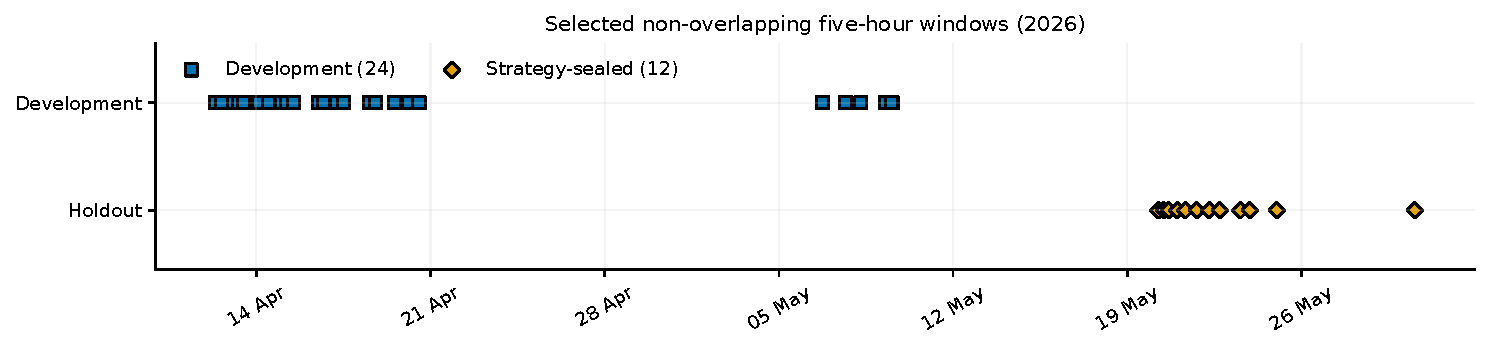
\includegraphics[width=0.96\textwidth]{../figures/panel_timeline.pdf}
\caption{Unchanged frozen selection used for V2 and corrected V3. The figure
is retained from the historical report because window membership did not
change. Holdout markers identify reserved windows, not evaluated strategies.}
\label{fig:panel}
\end{figure}

The V3 input audit verified all 240 selected spot depth/trade files against
their recorded SHA-256 values: 824,383,459 bytes in total. The inventory's
logical identity, the development CSV's byte hash, and the run's source hash
are distinct objects. They are listed in Appendix~\ref{sec:reproduction};
interchanging them would make a provenance check meaningless.

\subsection{Software responsibilities and flow}

\begin{figure}[H]
\centering
\begin{tikzpicture}[
  node distance=0.65cm and 0.55cm,
  box/.style={draw=Navy,rounded corners=2pt,fill=Pale,align=center,
    minimum height=0.95cm,text width=2.6cm,font=\small},
  arrow/.style={-{Latex[length=2mm]},thick,draw=Slate}]
\node[box] (raw) {Depth and trades\\with capture metadata};
\node[box,right=of raw] (parse) {Gap-aware parsers\\and stable merger};
\node[box,right=of parse] (book) {Book backend\\Python or C++};
\node[box,below=of parse] (replay) {Timestamp-batched\\Python replay};
\node[box,left=of replay] (strat) {Strategy intent\\and working risk};
\node[box,right=of replay] (exec) {Private scheduler\\queue, fills, fees};
\node[box,below=of replay] (analysis) {P\&L, markouts, OFI\\and uncertainty};
\node[box,right=of analysis] (outputs) {Hashed outputs\\and decision gate};
\draw[arrow] (raw)--(parse);
\draw[arrow] (parse)--(book);
\draw[arrow] (parse)--(replay);
\draw[arrow] (book)--(replay);
\draw[arrow] (replay)--(strat);
\draw[arrow] (strat)--(exec);
\draw[arrow] (exec)--(replay);
\draw[arrow] (replay)--(analysis);
\draw[arrow] (analysis)--(outputs);
\end{tikzpicture}
\caption{Research flow after native integration. The selected backend owns
book state; Python retains parsing, execution, strategy, and research
accounting. Native backend equivalence is assessed separately from the frozen
Python V3 experiment.}
\label{fig:architecture}
\end{figure}

\begin{table}[H]
\centering
\caption{The component boundaries make assumptions testable.}
\begin{tabularx}{\textwidth}{@{}L{0.29\textwidth}Y@{}}
\toprule
Component & Responsibility \\
\midrule
\code{src/replay/} & Decimal reference book, depth/trade parsers, event merge, timestamp groups, gap policy, and replay termination. \\
\code{src/execution/} & Private-order lifecycle, entry and cancel latency, post-only arrival, queue/FIFO transitions, fills, and fees. \\
\code{src/strategies/} & Symmetric and microprice quoting, blocked OFI-gated logic, tick rounding, requotes, and worst-case exposure. \\
\code{src/analysis/} & Accounting reconciliation, matched lots, forward marks, OFI/microprice regressions, bootstrap intervals, fee and tail diagnostics. \\
\code{scripts/} & Recording, panel orchestration, protocol validation, source/input identity, artifact verification, and report generation. \\
\code{cpp/} & Checked native book, canonical serialization, hashing, command-line interface, Python binding, and native tests. \\
\bottomrule
\end{tabularx}
\end{table}

Strategies request actions; they do not decide whether those actions have
arrived or filled. The execution simulator owns those transitions. Decimal
accounting and seeded independent entry/cancel randomness preserve repeatable
behavior. Canonical book hashes expose reconstruction divergence, while event
and accounting comparisons are needed to expose execution divergence. These
are complementary checks.
